\chapter{Design and Implementation}
\label{chap:design}
\section{Docker}
In native Docker, It has two part, Docker Client and Docker Daemon. Docker Daemon has many components include server, engine, registry, graph, driver and runC. To  support dump checkpoint and restore request, some of these steps should be implemented.

\subsection{Docker Client}
We implement 3 Docker commands in Docker Client, including checkpoint, restore, migrate. In checkpoint command should have these configurations:
\begin{itemize}
	\item image directory - Dump checkpoint image directory.
	\item work directory - Dump checkpoint image log directory.
	\item leave running - After dumping checkpoint image, keeping running container or not.
	\item pre-dump - Pre-dump checkpoint memory image to minimize frozen time.
	\item pre image directory - Define which version image to compare.
	\item track memory - Track memory to pre image directory image to minimize disk space.
\end{itemize}
In restore command should have these configurations:
\begin{itemize}
	\item image directory - Checkpoint image directory to restore from.
	\item work directory - Directory for restore log.
	\item force - Fore restoring container from image directory whether container is running or not.
\end{itemize}
In migrate command, it focus on Docker Swarm Scheduler filter configurations. In run command, we can do this with the environment variable or the label. Therefore, we implement environment variable and the label configurations in migrate command.

\subsection{Docker Daemon}
In native Docker Daemon, it doesn't support checkpoint and restore command.
Fortunately, it is already implemented in runC, so we have to add a proxy between Docker Daemon and runC, which can handle Docker Client's checkpoint and restore requests.

\section{Docker Swarm configuration}
As Figure \ref{fig:Docker Swarm with remote storage server}, we prepare a remote storage server for saving Docker containers dump checkpoint images. It should have fault tolerant to avoid service shout down. For these reasons, We choose glusterFS to be our experiments remote storage server.

\begin{figure}[h]
\begin{center}
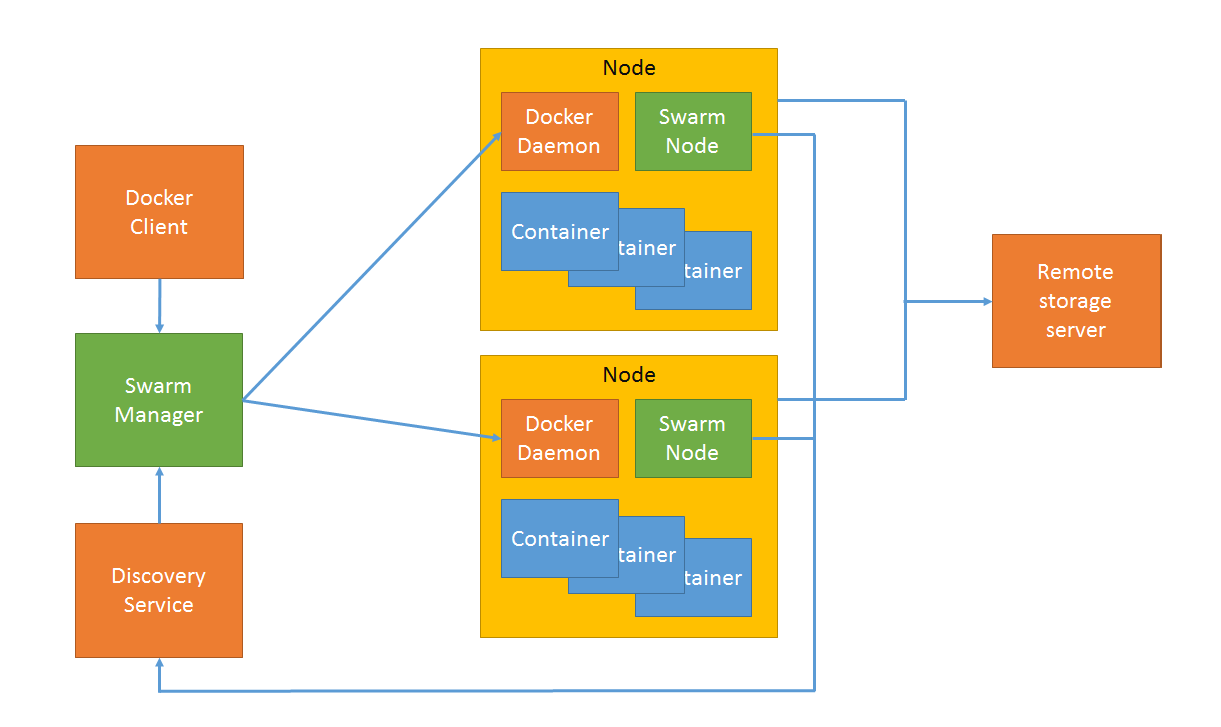
\includegraphics[width=15cm]{figure/swarm_docker_remote.png}
\end{center}
\caption{Docker Swarm with remote storage server}
\label{fig:Docker Swarm with remote storage server}
\end{figure}

\section{Docker containers migration in Docker Swarm}
Docker Swarm creates containers through Swarm scheduler to dispatch Docker nodes. If we want to specific assign which node we want to create containers, we have to set filters like constraint, affinity or dependency.
To migrate containers in Docker Swarm, we must avoid the containers which we want to migrate that migrate to an other nodes, instead of the same node.
\begin{enumerate}[Step 1.]
	\item Check Docker Swarm cluster has at least two Swarm nodes.
    \item Parse Docker Client requests to analyse label and environment variables, and transform label and environment variables to Docker Swarm filters.
    \item Add constraint filter to make sure the container which we want to migrate does not migrate to the same node.
    \item Create empty container on the Docker Swarm scheduler chooses node, this step could download the container image if it doesn't exist in the be chosen node.
    \item Pre-dump the container checkpoint image which we want to migrate to decrease container frozen time.
    \item Dump the container checkpoint image by tracking memory from pre-dump checkpoint image.
    \item Restore the container to the empty container that Docker Swarm scheduler chooses node.
    \item Delete the checkpoint images.
    \item If the container was migrated which had set checkpoint restore rescheduling policy, it will restart checkpoint restore rescheduling policy \ref{sec:checkpoint restore rescheduling policy}.
\end{enumerate}

\section{Docker Swarm checkpoint and restoration \\rescheduling policy}
\label{sec:checkpoint restore rescheduling policy}
In Docker Swarm, it has rescheduling policy. As we set the reschedule policy when we start a container, whenever Swarm nodes fail, Swarm Manager will restart the containers which on the fail nodes to another alive Swarm Nodes.

We improve this policy that we dump the checkpoint image for every containers which we want to keep the container checkpoint for every containers checkpoint ticker pounding. Whenever Swarm Nodes fail, Swarm Manager will restore the containers which Swarm Manager has dumped the checkpoint. Otherwise, the checkpoint tickers policy provides version of checkpoint image by tracking memory. It only dump different memory page checkpoint to new version checkpoint image.

In addition, it also support high availability that whenever Docker Swarm primary manager fails, the others Swarm Manager replica instances will lead a new primary manager. After replica leading a new primary manager, it will restart container checkpoint tickers.
%By experment, it can save at least XX% hard disk space

\subsection{Docker Swarm Container Checkpoint Tickers Strategy}
The details of our algorithm in Algorithm \ref{code:checkpointTicker} that explains Container Checkpoint Tickers Strategy.
In line1 and line2, we set checkpoint-time $T_i$ and version-group $VG_i$ when we create the container $C_i$ through Docker Swarm Manager, and every $T_i$ are independent.
Each $T_i$ in the Docker Swarm cluster has its starting time and time ticker, time ticker will dump checkpoint image repeatedly at regular intervals. If version-group $VG_i$ doesn't be set, it will be set to 5.
We define checkpoint version $V_i=0$, and pre-dump checkpoint version $pre$-$dump V_i=0$ for each container $C_i$.

In line4-18, for each container is running and $C_i$ checkpoint ticker $T_i$ is time up, $C_i$, Swarm Manger will do line5-17.
In line6-9, if the container $C_i$ doesn't has any pre-dump image or newest version-group $VG_i$ checkpoint is full, Swarm Manger will send the request to Swarm Node $N_i$ to create a new directory and pre-dump the checkpoint image as pre-dump version $pre$-$dump V_i$.
After pre-dumping the container checkpoint image or $C_i$ has previous version checkpoint images, Swarm Manager sends request to dump checkpoint image to Swarm Node $N_i$ to dump checkpoint version $V_i$. Whenever dumping checkpoint image, CRIU will track memory different to the previous checkpoint image or the pre-dumping checkpoint image do reduce image dick space. As is shown as Figure \ref{fig:Containers checkpoint versions in remote storage server}, every container has each pre-dump checkpoint directories and each pre-dump checkpoint directories has version-group versions checkpoint images.
In line10-12, Swarm Manager Sends delete checkpoint request to $N_i$ to delete oldest Pre-dump version directory whenever container has more than three Pre-dump versions directory. 

\begin{figure}[h]
\begin{center}
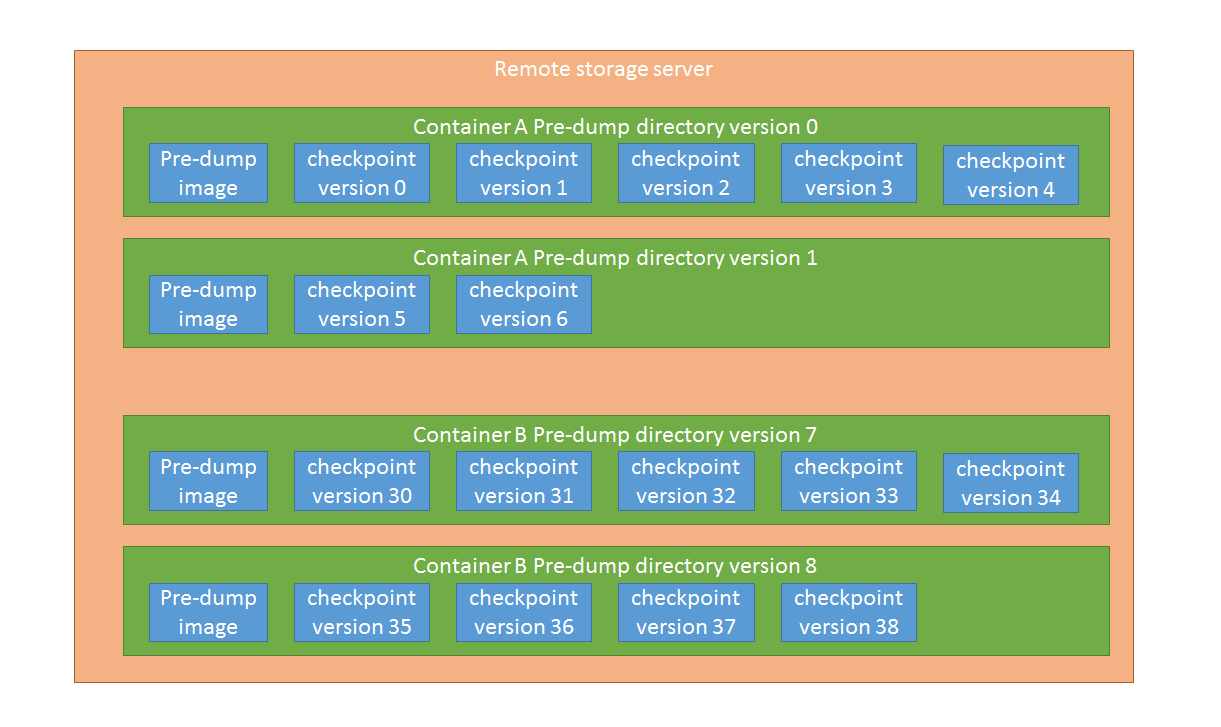
\includegraphics[width=15cm]{figure/checkpoint_demo.png}
\end{center}
\caption{Containers checkpoint versions in remote storage server}
\label{fig:Containers checkpoint versions in remote storage server}
\end{figure}

\begin{algorithm}[h]
    \caption{Checkpoint ticker algorithm}
    \label{code:checkpointTicker}
    \begin{algorithmic}[1]
	\Require
		The set of Swarm Nodes: $\lbrace N_1,N_2,...,N_m \rbrace $;
		The set of containers: $\lbrace C_1,C_2,...,C_n \rbrace$;
		Version-group: $ VG_i $;
		Checkpoint-ticker time: $ T_i $;
	\Ensure
		pre-dump images $ pre$-$dump V_i $; dump images $ V_i $ ;
        \State Set $ T_i $ and $ VG_i $ labels when create the container $ C_i $;
        \State initial $ V_i=0 $, $ pre$-$dump V_i=0 $;
        \\
        \For {each $ C_i $ in $ N_i $}
        	\While {$ C_i $ running $ \& $ $ T_i $ pounding}
            	\If {version $ \% $ $ VG_i $ == 0 } 
					\State pre-dump checkpoint image $ pre $-$ dump V_i $;
				\EndIf
			\State dump checkpoint image $ V_i $;
				\If { $ VG_i$ directory $ > $ 3 } 
                	\State delete oldest pre-dump checkpoint $ pre $-$ dump V_i $ directory;
				\EndIf
            	\State $ V_i $ = $ V_ i$ + 1;
            	\If {$ V_i $ $\%$ $VG_i$ == 0 } 
          	      \State $ pre $-$ dump V_i $ = $ pre $-$ dump V_i $ + 1;
        	    \EndIf
     	   \EndWhile
        \EndFor
    \end{algorithmic}
\end{algorithm}

\subsection{Docker Swarm Restore Rescheduling Policy}
Algorithm \ref{code:Restore} gives a detailed explanation of restore Rescheduling Policy. In line1, we set $ R_i $ label when we create the container $C_i$ through Docker Swarm Manager. In line3-7, Whenever Swarm Nodes $ N_i $ fail, Swarm Manager will execute procedure \textsc{Restore container} that restore every containers $ C_i $ which has $ R_i $ label to another Swarm Nodes $ N_i $.

In line9-21, each container $ C_i $ executes procedure \textsc{Restore container}, Swarm Manager will choose a Swarm Node $ N_r $ and create an empty container $ C_r $ in $ N_r $. In this step, Swarm Manager will check $ N_r $ has container image or not, if $ N_r $ doesn't have container image, $ N_r $ will download the container image from Docker remote registry and create the empty container $ C_r $.
As a result of creating container $ C_r $, Swarm Manager restores the fail container $ C_i $ checkpoint image to $ C_r $. To avoid restoring fail, Swarm Manager will retry second last version checkpoint to restore, and it will retry version-group(default is 5) times. The container $ C_i $ checkpoint image will be delete after restoring the container  $ C_i $.

If Swarm Manager retries version-group all fail, it will create and start a new container as normal Docker Swarm rescheduling policy.

\begin{algorithm}[h]
    \caption{Restore rescheduling policy algorithm}
    \label{code:Restore}
    \begin{algorithmic}[1]
    	\Require
		The set of Swarm Nodes: $ \lbrace N_1,N_2,...,N_m \rbrace $;
		The set of containers: $ \lbrace C_1,C_2,...,C_n \rbrace $;
		Version-group: $ VG_i $;
		Checkpoint-ticker time: $ T_i $;
		Restore rescheduling policy label:$ R_i $;
	\Ensure
		Restored containers:$ C_{ri} $;
        \State Set $ R_i $ labels create the container;
        \\
        \If {$ N_i $ fail}
        	\ForAll{$ C_i $ in fail $N_i$ has $ R_i $}
        		\State \textsc{Restore Container};
        	\EndFor
        \EndIf
        \\
        \Procedure{Restore Container}{}
			\State $ N_r $ $\longleftarrow$Create a empty container $ C_r $
			\For {$ V_i $ downto $ V_i $ - $ VG_i $}
				\State $ C_{ri} $ $\longleftarrow$ Restore checkpoint $ V_i $;
				\If{ Restore $ C_{ri} $ success }
					\State \textbf{break}
				\EndIf
			\EndFor
			\State Delete the container checkpoint image;
			\If{Restore container $C_i$ fail}
				\State $ C_r \longleftarrow $ Restart the container; $C_i$;
			\EndIf
		\EndProcedure
	\end{algorithmic}
\end{algorithm}
\subsection{High availability of Swarm Manager in Docker Swarm checkpoint and restoration rescheduling policy}
Whenever Docker Swarm primary manager fails, the others Swarm Manager replica instances will lead a new primary manager. After replica leading a new primary manager, it searching every Docker Node's containers which has checkpoint restore rescheduling policy's label. If the containers has checkpoint restore rescheduling policy's label, Docker Swarm new primary manager will restart container checkpoint tickers.